\documentclass[13pt,onlymath]{beamer}
\usefonttheme{serif}
\usepackage{graphicx,amsmath,amssymb,tikz,psfrag,epstopdf,fancyvrb}
\usepackage[lighttt]{lmodern}
%\usepackage{graphicx,psfrag}

\input defs.tex

%% formatting

\mode<presentation>
{
\usetheme{default}
}
\setbeamertemplate{navigation symbols}{}
\usecolortheme[rgb={0.13,0.28,0.59}]{structure}
\setbeamertemplate{itemize subitem}{--}
\setbeamertemplate{frametitle} {
    \begin{center}
      {\large\bf \insertframetitle}
    \end{center}
}

\newcommand\footlineon{
  \setbeamertemplate{footline} {
    \begin{beamercolorbox}[ht=2.5ex,dp=1.125ex,leftskip=.8cm,rightskip=.6cm]{structure}
      \footnotesize \insertsection
      \hfill
      {\insertframenumber}
    \end{beamercolorbox}
    \vskip 0.45cm
  }
}
\footlineon

\AtBeginSection[] 
{ 
    \begin{frame}<beamer> 
        \frametitle{Outline} 
        \tableofcontents[currentsection,currentsubsection] 
    \end{frame} 
} 

%% begin presentation

\title{\large \bfseries String Algorithms}

\author{Jaehyun Park\\[3ex]
CS 97SI\\
Stanford University}

\date{\today}

\begin{document}

\frame{
\thispagestyle{empty}
\titlepage
}

\section{String Matching Problem}

\begin{frame}{String Matching Problem}
\BIT
\item Given a text $T$ and a pattern $P$, find all occurrences of $P$ within $T$
\item Notations:
\BIT
\item $n$ and $m$: lengths of $P$ and $T$
\item $\Sigma$: set of alphabets (of constant size)
\item $P_i$: $i$th letter of $P$ (1-indexed)
\item $a$, $b$, $c$: single letters in $\Sigma$
\item $x$, $y$, $z$: strings
\EIT \EIT
\end{frame}

\begin{frame}{Example}
\BIT
\item $T = \mathtt{AGCATGCTGCAGTCATGCTTAGGCTA}$
\item $P = \mathtt{GCT}$
\item $P$ appears three times in $T$
\vfill
\item A naive method takes $O(mn)$ time
\BIT
\item Initiate string comparison at every starting point
\item Each comparison takes $O(m)$ time
\EIT
\vfill
\item We can do much better!
\EIT
\end{frame}


\section{Hash Table}

\begin{frame}{Hash Function}
\BIT
\item A function that takes a string and outputs a number
\item A good hash function has few collisions
\BIT
\item \ie, If $x\ne y$, $H(x) \ne H(y)$ with high probability
\EIT
\item An easy and powerful hash function is a polynomial mod some prime $p$
\BIT
\item Consider each letter as a number (ASCII value is fine)
\item $H(x_1 \ldots x_k) = x_1 a^{k-1} + x_2 a^{k-2} + \cdots + x_{k-1} a + x_k \pmod{p}$
\item How do we find $H(x_2 \ldots x_{k+1})$ from $H(x_1 \ldots x_k)$?
\EIT\EIT
\end{frame}

\begin{frame}{Hash Table}
\BIT
\item Main idea: preprocess $T$ to speedup queries
\BIT
\item Hash every substring of length $k$
\item $k$ is a small constant
\EIT
\vfill
\item For each query $P$, hash the first $k$ letters of $P$ to retrieve all the occurrences of it within $T$
\vfill
\item Don't forget to check collisions!
\EIT
\end{frame}

\begin{frame}{Hash Table}
\BIT
\item Pros:
\BIT
\item Easy to implement
\item Significant speedup in practice
\EIT
\vfill
\item Cons:
\BIT
\item Doesn't help the asymptotic efficiency
\BIT
\item Can still take $\Theta(nm)$ time if hashing is terrible or data is difficult
\EIT
\item A lot of memory consumption
\EIT\EIT
\end{frame}


\section{Knuth-Morris-Pratt (KMP) Algorithm}

\begin{frame}{Knuth-Morris-Pratt (KMP) Matcher}
\BIT
\item A linear time (!) algorithm that solves the string matching problem by preprocessing $P$ in $\Theta(m)$ time
\BIT
\item Main idea is to skip some comparisons by using the previous comparison result
\EIT
\item Uses an auxiliary array $\pi$ that is defined as the following:
\BIT
\item $\pi[i]$ is the largest integer smaller than $i$ such that $P_1 \ldots P_{\pi[i]}$ is a suffix of $P_1 \ldots P_i$
\EIT
\item ... It's better to see an example than the definition
\EIT
\end{frame}

\begin{frame}{$\pi$ Table Example (from CLRS)}
\begin{center}
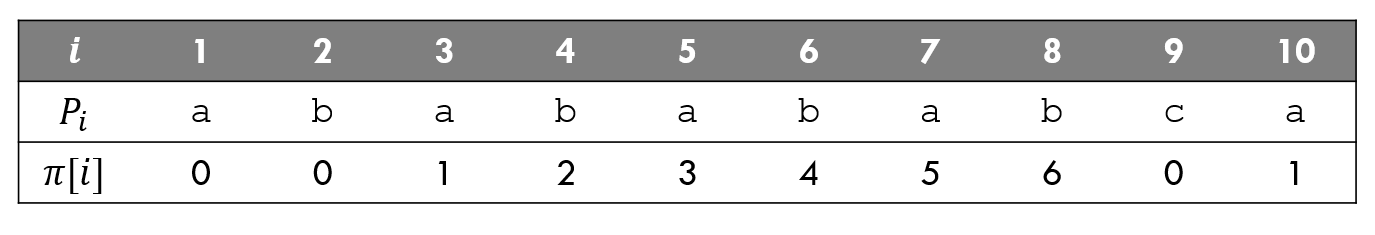
\includegraphics[width=0.9\textwidth]{figures/pitable}
\end{center}
\BIT
\item $\pi[i]$ is the largest integer smaller than $i$ such that $P_1 \ldots P_{\pi[i]}$ is a suffix of $P_1 \ldots P_i$
\BIT
\item \eg, $\pi[6]=4$ since \texttt{abab} is a suffix of \texttt{ababab}
\item \eg, $\pi[9]=0$ since no prefix of length $\le 8$ ends with $c$
\EIT
\item Let's see why this is useful
\EIT
\end{frame}

\begin{frame}{Using the $\pi$ Table}
\BIT
\item $T=\mathtt{ABC\:\;ABCDAB\:\;ABCDABCDABDE}$
\item $P=\mathtt{ABCDABD}$
\item $\pi = (0,0,0,0,1,2,0)$
\item Start matching at the first position of $T$:
\begin{center}
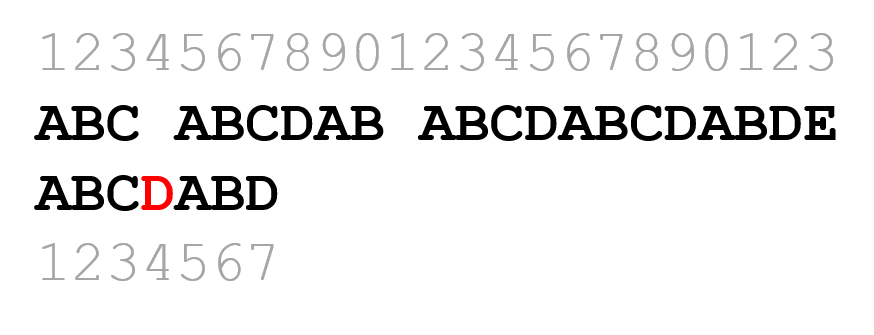
\includegraphics[width=0.7\textwidth]{figures/kmp1}
\end{center}
\item Mismatch at the 4th letter of $P$!
\EIT
\end{frame}

\begin{frame}{Using the $\pi$ Table}
\BIT
\item We matched $k=3$ letters so far, and $\pi[k] = 0$
\BIT
\item Thus, there is no point in starting the comparison at $T_2$, $T_3$ (crucial observation)
\EIT
\item Shift $P$ by $k-\pi[k] = 3$ letters
\begin{center}
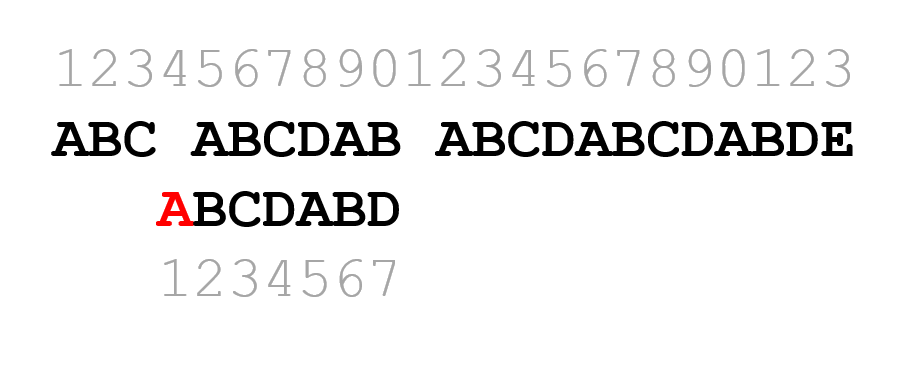
\includegraphics[width=0.7\textwidth]{figures/kmp2}
\end{center}
\item Mismatch at $T_4$ again!
\EIT
\end{frame}

\begin{frame}{Using the $\pi$ Table}
\BIT
\item We matched $k=0$ letters so far
\item Shift $P$ by $k-\pi[k] = 1$ letter (we define $\pi[0] = -1$)
\begin{center}
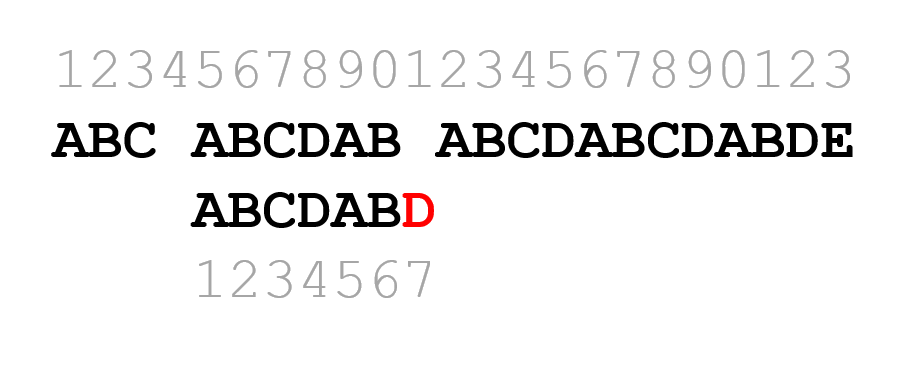
\includegraphics[width=0.7\textwidth]{figures/kmp3}
\end{center}
\item Mismatch at $T_{11}$!
\EIT
\end{frame}

\begin{frame}{Using the $\pi$ Table}
\BIT
\item $\pi[6]=2$ means $P_1 P_2$ is a suffix of $P_1 \ldots P_6$
\item Shift $P$ by $6 - \pi[6] = 4$ letters
\begin{center}
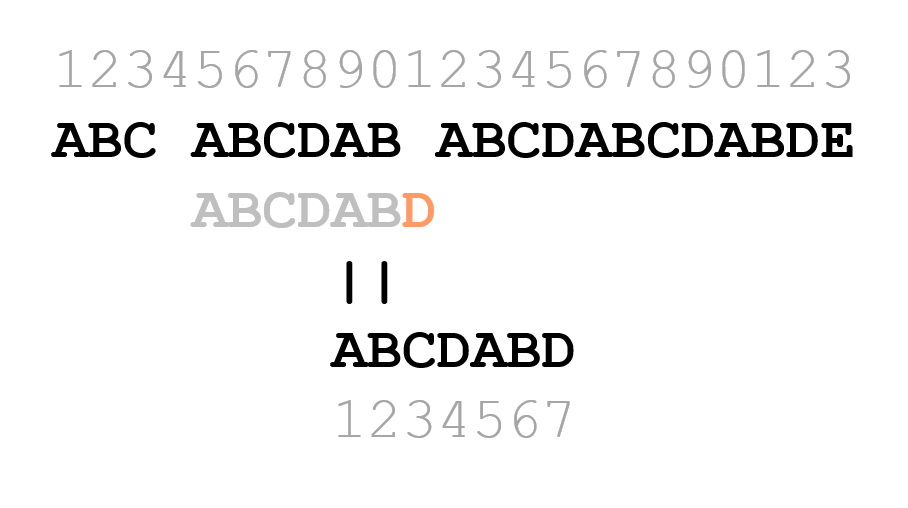
\includegraphics[width=0.7\textwidth]{figures/kmp4}
\end{center}
\item Again, no point in shifting $P$ by 1, 2, or 3 letters
\EIT
\end{frame}

\begin{frame}{Using the $\pi$ Table}
\BIT
\item Mismatch at $T_{11}$ again!
\begin{center}
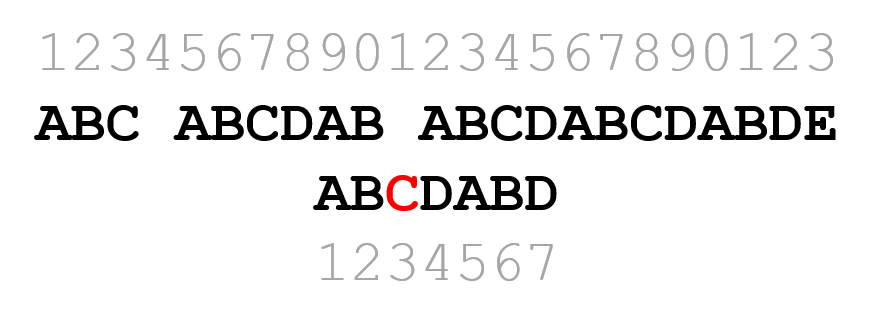
\includegraphics[width=0.7\textwidth]{figures/kmp5}
\end{center}
\item Currently 2 letters are matched
\item Shift $P$ by $2-\pi[2] = 2$ letters
\EIT
\end{frame}

\begin{frame}{Using the $\pi$ Table}
\BIT
\item Mismatch at $T_{11}$ yet again!
\begin{center}
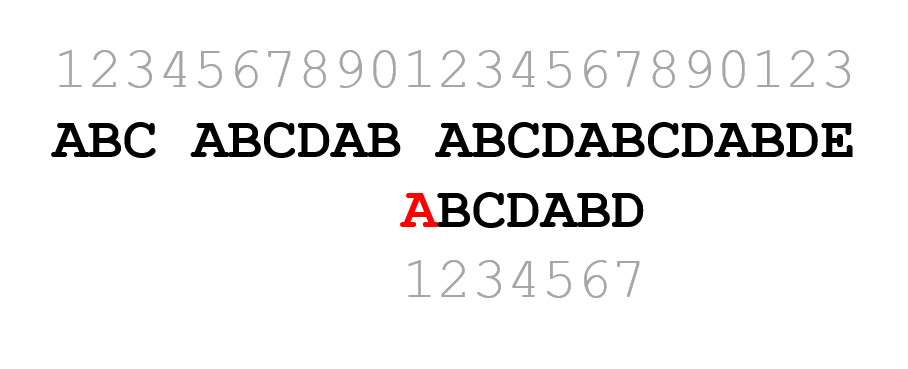
\includegraphics[width=0.7\textwidth]{figures/kmp6}
\end{center}
\item Currently no letters are matched
\item Shift $P$ by $0-\pi[0] = 1$ letter
\EIT
\end{frame}

\begin{frame}{Using the $\pi$ Table}
\BIT
\item Mismatch at $T_{18}$
\begin{center}
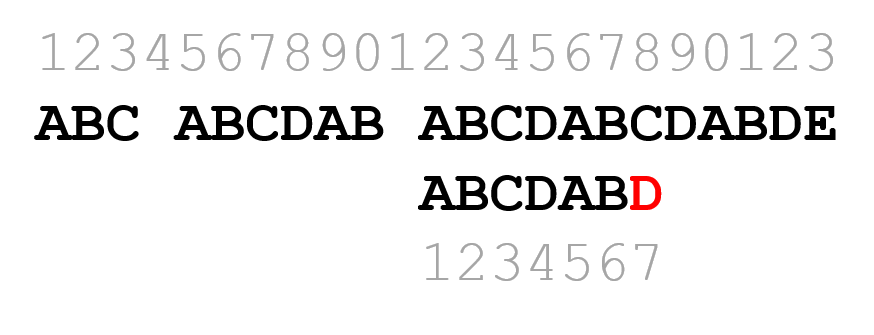
\includegraphics[width=0.7\textwidth]{figures/kmp7}
\end{center}
\item Currently 6 letters are matched
\item Shift $P$ by $6-\pi[6] = 4$ letters
\EIT
\end{frame}

\begin{frame}{Using the $\pi$ Table}
\BIT
\item Finally, there it is!
\begin{center}
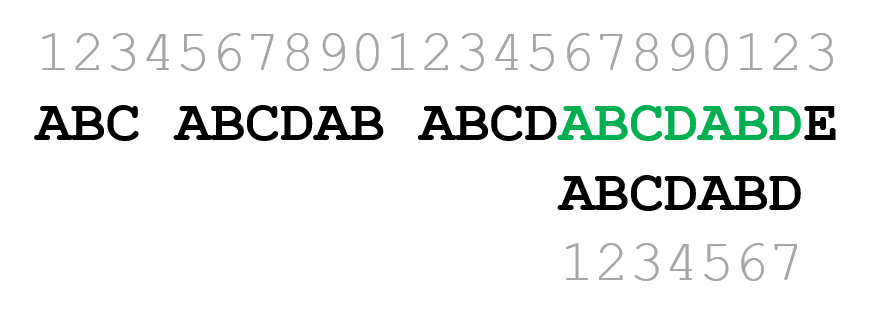
\includegraphics[width=0.7\textwidth]{figures/kmp8}
\end{center}
\item Currently all 7 letters are matched
\item After recording this match (at $T_{16} \ldots T_{22}$, we shift $P$ again in order to find other matches
\BIT
\item Shift by $7-\pi[7] = 7$ letters
\EIT\EIT
\end{frame}

\begin{frame}{Computing $\pi$}
\BIT
\item Observation 1: if $P_1\ldots P_{\pi[i]}$ is a suffix of $P_1 \ldots P_i$, then $P_1 \ldots P_{\pi[i]-1}$ is a suffix of $P_1 \ldots P_{i-1}$
\BIT
\item Well, obviously...
\EIT
\item Observation 2: all the prefixes of $P$ that are a suffix of $P_1 \ldots P_i$ can be obtained by recursively applying $\pi$ to $i$
\BIT
\item \eg, $P_1 \ldots P_{\pi[i]}$, $P_1 \ldots, P_{\pi[\pi[i]]}$, $P_1 \ldots, P_{\pi[\pi[\pi[i]]]}$ are all suffixes of $P_1 \ldots P_i$
\EIT \EIT
\end{frame}

\begin{frame}{Computing $\pi$}
\BIT
\item A non-obvious conclusion:
\BIT
\item First, let's write $\pi^{(k)}[i]$ as $\pi[\cdot]$ applied $k$ times to $i$
\item \eg, $\pi^{(2)}[i] = \pi[\pi[i]]$
\item $\pi[i]$ is equal to $\pi^{(k)}[i-1] + 1$, where $k$ is the smallest integer that satisfies $P_{\pi^{(k)}[i-1]+1} = P_i$
\BIT
\item If there is no such $k$, $\pi[i] = 0$
\EIT\EIT
\item Intuition: we look at all the prefixes of $P$ that are suffixes of $P_1 \ldots P_{i-1}$, and find the longest one whose next letter matches $P_i$
\EIT
\end{frame}

\begin{frame}[fragile]{Implementation}
\begin{Verbatim}[xleftmargin=25pt]
pi[0] = -1;
int k = -1;
for(int i = 1; i <= m; i++) {
  while(k >= 0 && P[k+1] != P[i])
    k = pi[k];
  pi[i] = ++k;
}
\end{Verbatim}
\end{frame}

\begin{frame}[fragile]{Pattern Matching Implementation}
\begin{Verbatim}[xleftmargin=25pt]
int k = 0;
for(int i = 1; i <= n; i++) {
  while(k >= 0 && P[k+1] != T[i])
    k = pi[k];
  k++;
  if(k == m) {
    // P matches T[i-m+1..i]
    k = pi[k];
  }
}
\end{Verbatim}
\end{frame}

\section{Suffix Trie}

\begin{frame}{Suffix Trie}
\BIT
\item Suffix trie of a string $T$ is a rooted tree that stores all the suffixes (thus all the substrings)
\item Each node corresponds to some substring of $T$
\item Each edge is associated with an alphabet
\item For each node that corresponds to $ax$, there is a special pointer called \emph{suffix link} that leads to the node corresponding to $x$
\item Surprisingly easy to implement!
\EIT
\end{frame}

\begin{frame}{Example}
\begin{center}
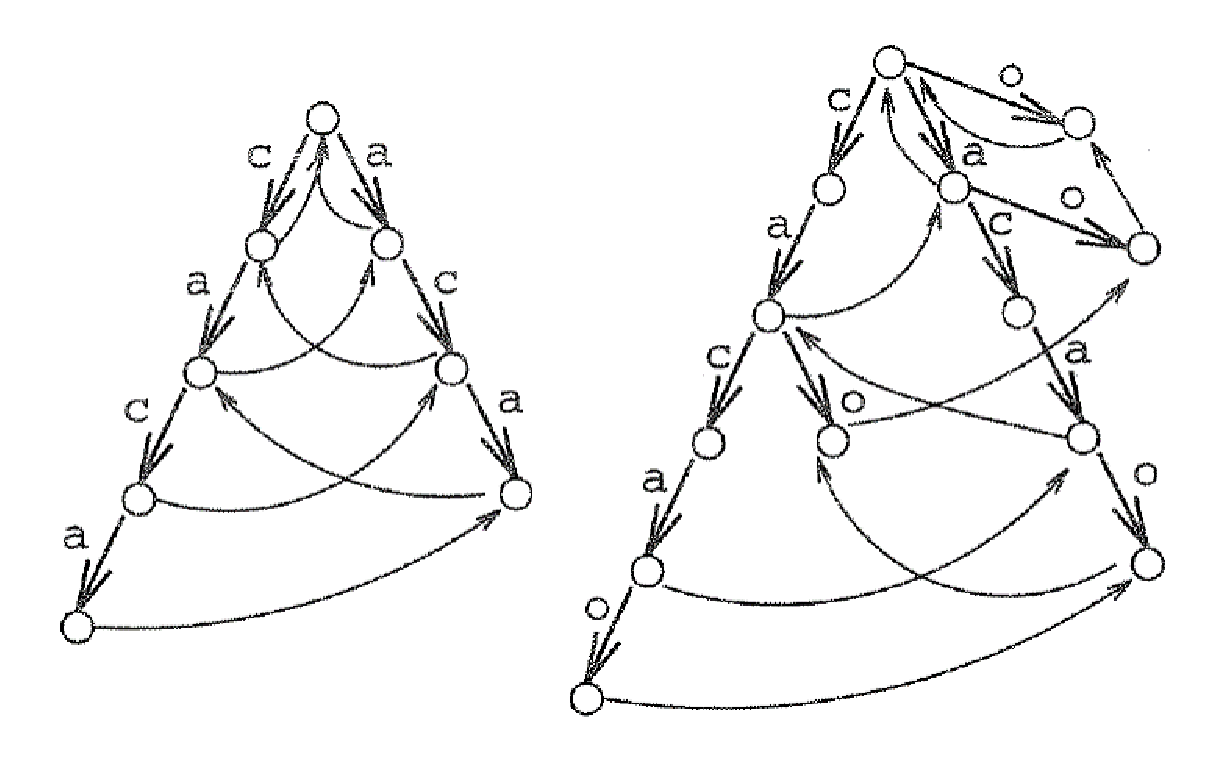
\includegraphics[width=0.7\textwidth]{figures/suftrie}

(Figure modified from Ukkonen's original paper)
\end{center}
\end{frame}

\begin{frame}{Incremental Construction}
\BIT
\item Given the suffix tree for $T_1 \ldots T_n$
\BIT
\item Then we append $T_{n+1} = a$ to $T$, creating necessary nodes
\EIT
\item Start at node $u$ corresponding to $T_1 \ldots T_n$
\BIT
\item Create an $a$-transition to a new node $v$
\EIT
\item Take the suffix link at $u$ to go to $u'$, corresponding to $T_2 \ldots T_n$
\BIT
\item Create an $a$-transition to a new node $v'$
\item Create a suffix link from $v$ to $v'$
\EIT\EIT
\end{frame}

\begin{frame}{Incremental Construction}
\BIT
\item Repeat the previous process:
\BIT
\item Take the suffix link at the current node
\item Make a new $a$-transition there
\item Create the suffix link from the previous node
\EIT
\item Stop if the node already has an $a$-transition
\BIT
\item Because from this point, all nodes that are reachable via suffix links already have an $a$-transition
\EIT\EIT
\end{frame}

\begin{frame}{Construction Example}
\begin{center}
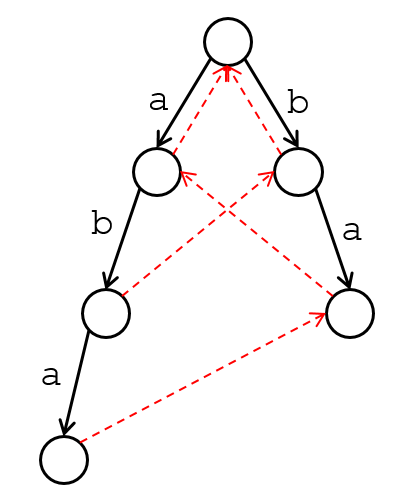
\includegraphics[height=0.5\textheight]{figures/trie1}

Given the suffix trie for \texttt{aba}\\
We want to add a new letter \texttt{c}
\end{center}
\end{frame}

\begin{frame}{Construction Example}
\begin{center}
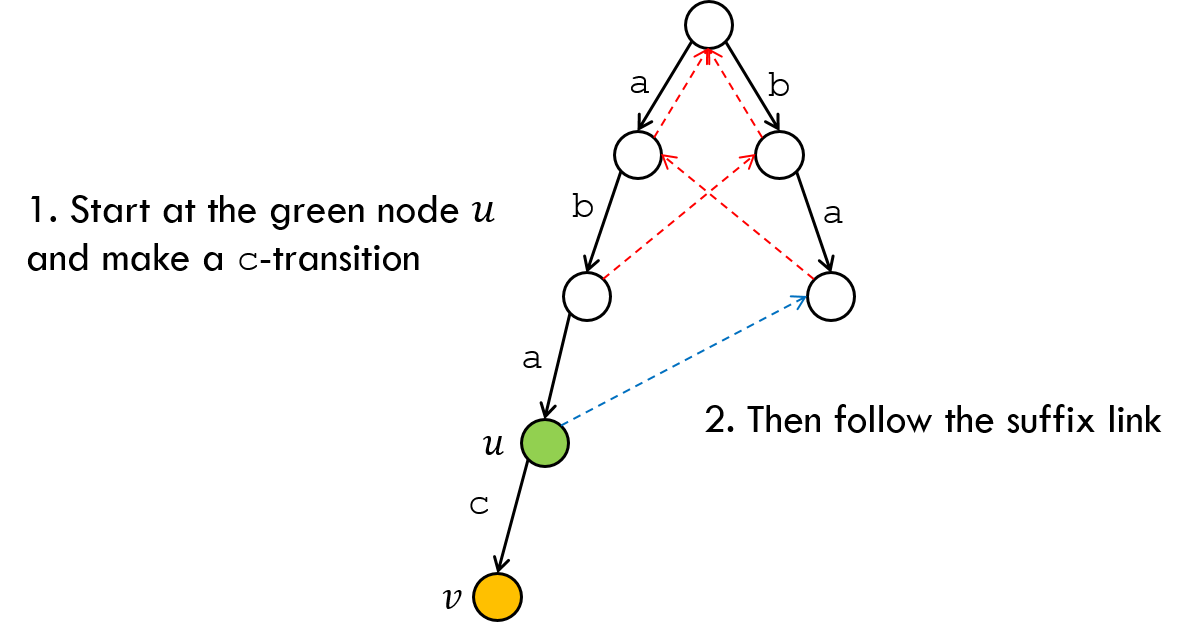
\includegraphics[height=0.5\textheight]{figures/trie2}
\end{center}
\end{frame}

\begin{frame}{Construction Example}
\begin{center}
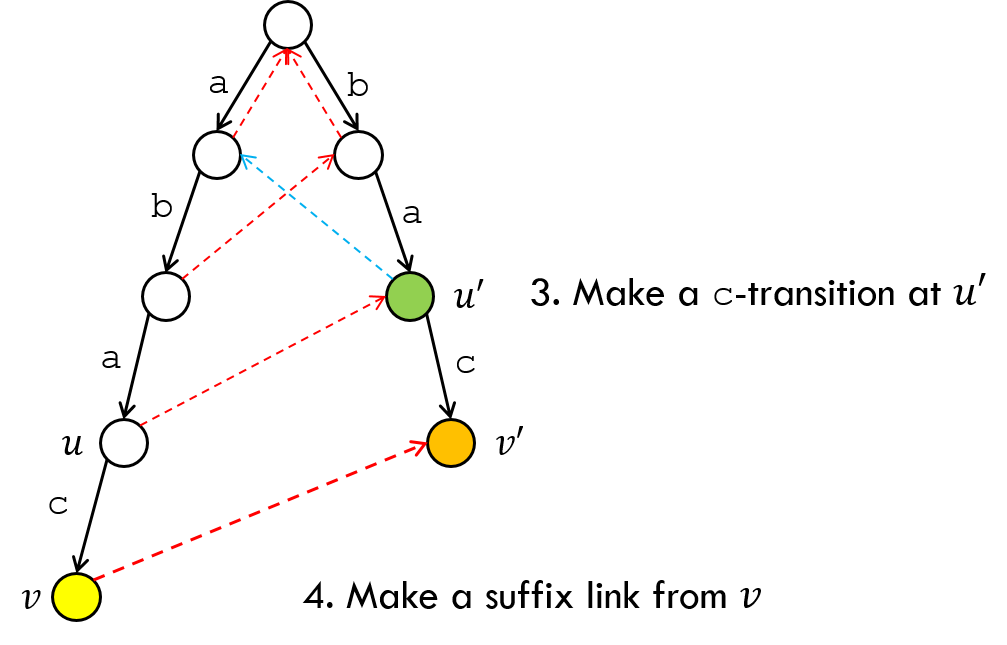
\includegraphics[height=0.5\textheight]{figures/trie3}
\end{center}
\end{frame}

\begin{frame}{Construction Example}
\begin{center}
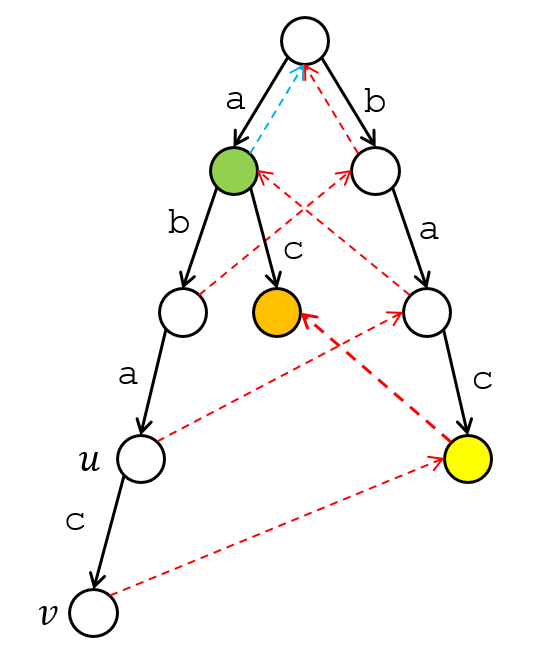
\includegraphics[height=0.5\textheight]{figures/trie4}
\end{center}
\end{frame}

\begin{frame}{Construction Example}
\begin{center}
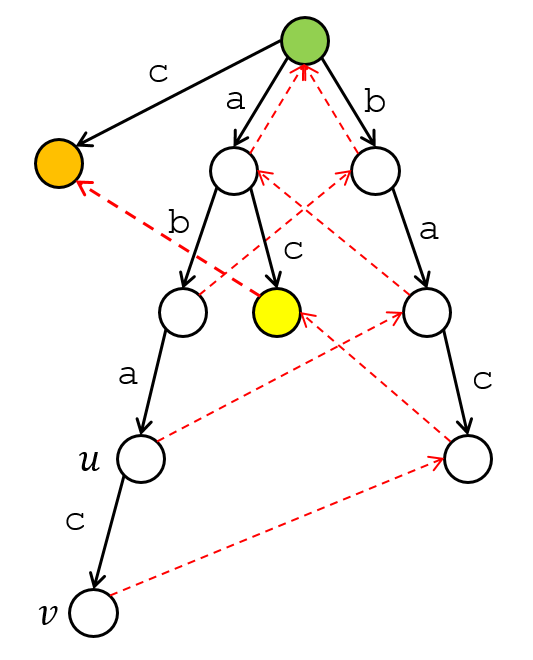
\includegraphics[height=0.5\textheight]{figures/trie5}
\end{center}
\end{frame}

\begin{frame}{Construction Example}
\begin{center}
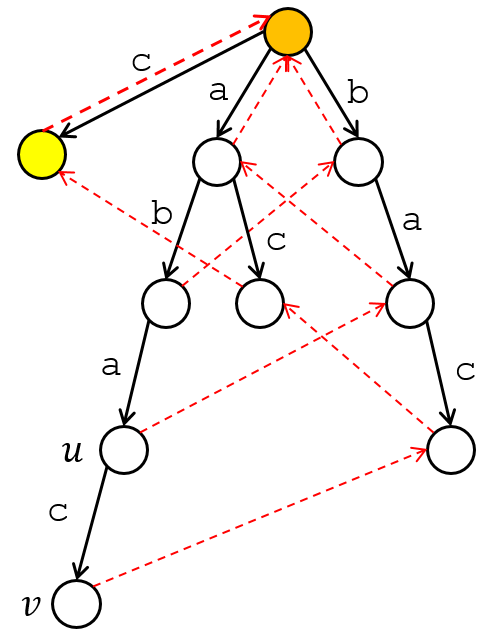
\includegraphics[height=0.5\textheight]{figures/trie6}
\end{center}
\end{frame}

\begin{frame}{Construction Example}
\BIT
\item Construction time is linear in the tree size
\item But the tree size can be quadratic in $n$
\BIT
\item \eg, $T = \mathtt{aa}\ldots\mathtt{abb}\ldots\mathtt{b}$
\EIT\EIT
\end{frame}

\begin{frame}{Construction Example}
\BIT
\item To find $P$, start at the root and keep following edges labeled with $P_1$, $P_2$, etc.
\vfill
\item Got stuck? Then $P$ doesn't exist in $T$
\EIT
\end{frame}



\section{Suffix Array}

\begin{frame}{Suffix Array}
\begin{center}
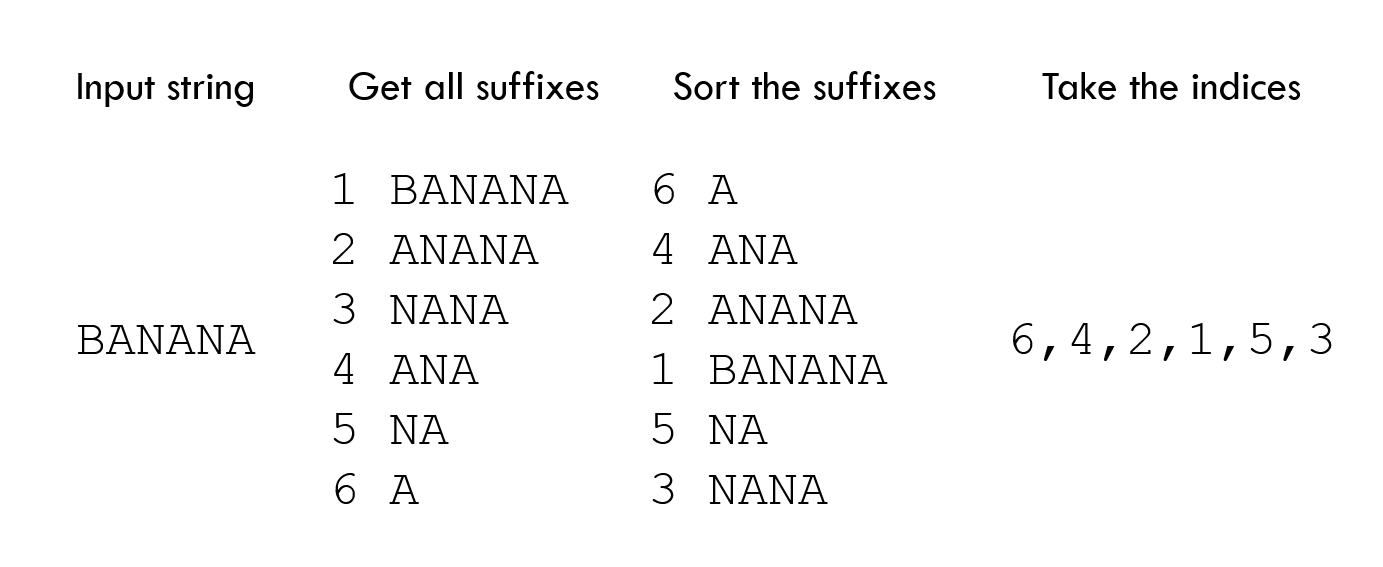
\includegraphics[width=0.8\textwidth]{figures/sufarray}
\end{center}
\end{frame}

\begin{frame}{Suffix Array}
\BIT
\item Memory usage is $O(n)$
\item Has the same computational power as suffix trie
\item Can be constructed in $O(n)$ time (!)
\BIT
\item But it's hard to implement
\EIT
\item There is an approachable $O(n \log^2 n)$ algorithm
\BIT
\item If you want to see how it works, read the paper on the course website
\item \url{http://cs97si.stanford.edu/suffix-array.pdf}
\EIT\EIT
\end{frame}


\begin{frame}{Notes on String Problems}
\BIT
\item Always be aware of the null-terminators
\item Simple hash works so well in many problems
\item If a problem involves rotations of some string, consider concatenating it with itself and see if it helps
\item Stanford team notebook has implementations of suffix arrays and the KMP matcher
\EIT
\end{frame}


\end{document}
